% !TeX program = xelatex
% !TeX encoding = UTF-8
\documentclass[UTF8]{standalone}
\usepackage{amsmath,fourier,ctex,tikz}
\begin{document}
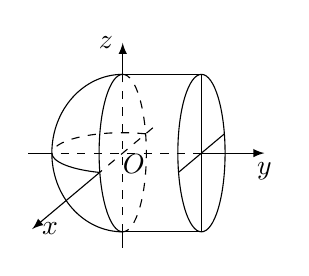
\begin{tikzpicture}
	\draw[dashed] (-1,0) -- (1,0);
	\draw[dashed] (40:0.5) -- (-140:0.38);
	\draw (1,0) ellipse (0.3 and 1);
	\draw (1,0) ++ (-140:0.38) -- ++ (40:0.76);
	\draw (0,1) arc [start angle=90, end angle=270, x radius=0.3, y radius=1];
	\draw[dashed] (0,1) arc [start angle=90, end angle=-90, x radius=0.3, y radius=1];
	\draw (0,1) arc [start angle=90, end angle=270, x radius=0.9, y radius=1];
	\draw (0,1) -- ++ (1,0);
	\draw (0,-1) -- ++ (1,0);
	\draw (1,1) -- ++ (0,-2);
	\draw[dashed] (40:0.38) arc [start angle=71, end angle=180, x radius=0.9, y radius=0.27];
	\draw (-0.9,0) arc [start angle=180, end angle=251, x radius=0.9, y radius=0.26];
	\draw[-latex] (-140:0.38) -- (-140:1.5) node[right] {$x$};
	\draw[dashed] (0,-1) -- node[right=4pt,below=-3pt] {$O$} (0,1);
	\draw (0,-1) -- ++(0,-0.2);
	\draw[-latex] (0,1) -- ++ (0,0.4) node[left] {$z$};
	\draw[-latex] (1,0) -- ++(0.8,0) node[below] {$y$};
	\draw (-0.9,0) -- ++ (-0.3,0);
\end{tikzpicture}
\end{document}